\section{
زمان‌بندی پروژه
}

\subsection*{
ضرب الاجل‌های اصلی
}

\begin{itemize}
	\item{
		\textbf{
یکم آبان ماه ۱۴۰۰:
		}
آغاز پروژه
	}
	\item{
	\textbf{پانزدهم آبان ماه ۱۴۰۰:}	
	وظایف اعضای تیم می‌بایست مشخص شده باشد و طراحی اولیه از تمام سیستم ارائه شود.
	}
	\item{
\textbf{سی ام آ‌ذر ماه ۱۴۰۰:}
پایان توسعه سیستم و نگارش اسناد.	
	}
	\item{
\textbf{ پانزدهم دی ماه ۱۴۰۰}	
پایان نصب و راه اندازی سیستم و در اختیار قرارگیری آن و همچنین رفع مشکلات احتمالی گزارش شده توسط کاربران.
	}
	\item{
\textbf{یکم بهمن ماه ۱۴۰۰}
تحویل کامل پروژه و اتمام پروژه	
	}
	
	
\end{itemize}

\subsection*{
نمودار گانت چارت
}

\begin{center}
  \begin{figure} [h!]
    { 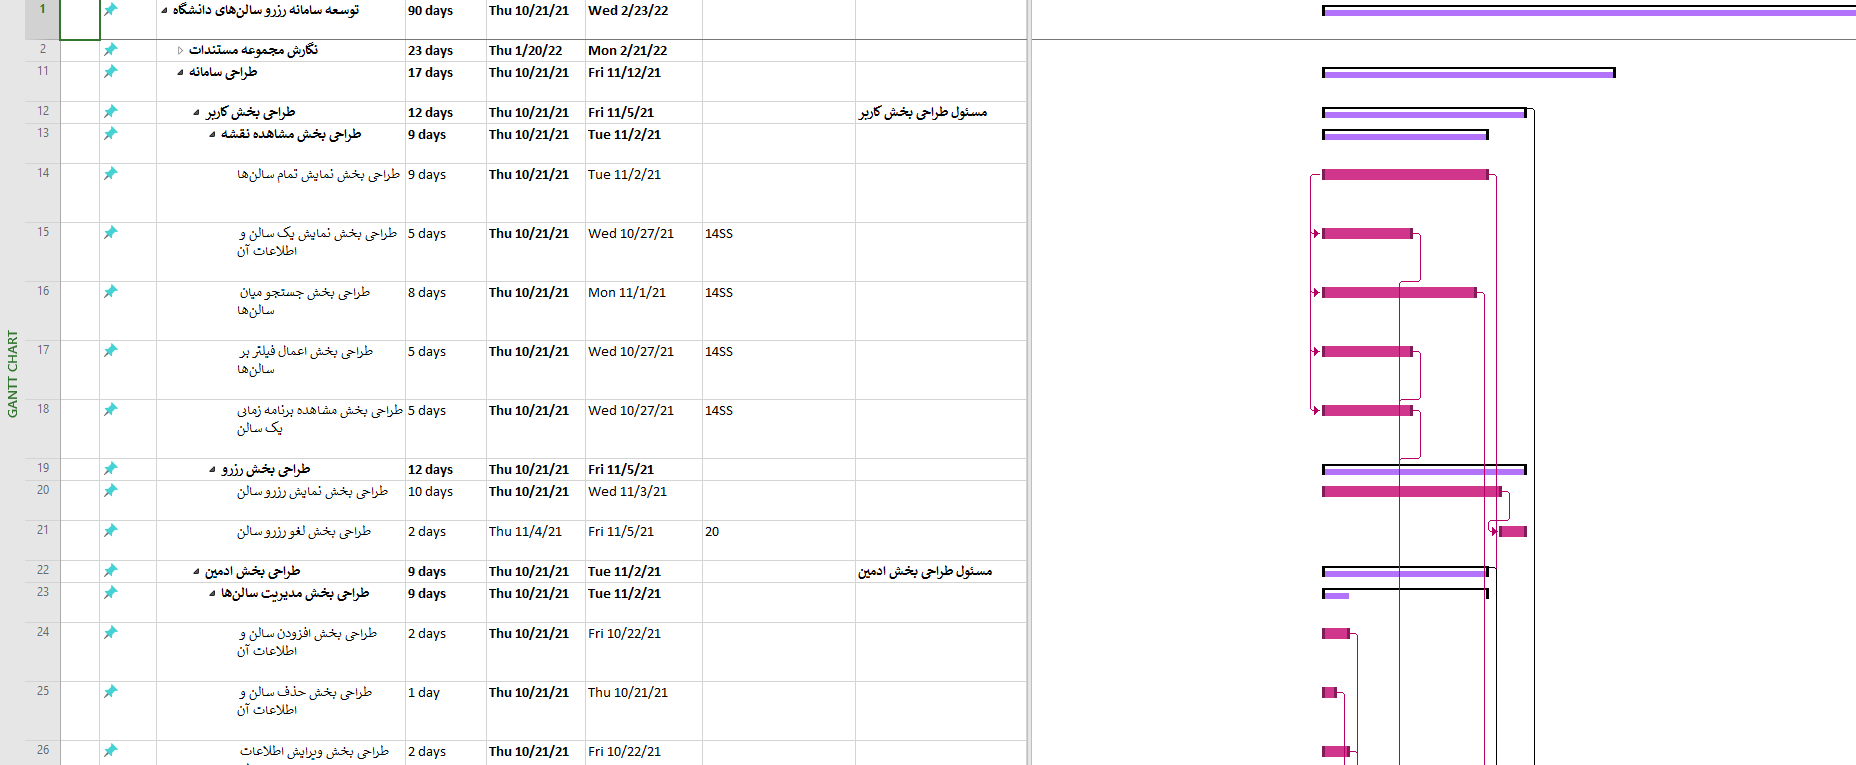
\includegraphics[width=\textwidth]{appandecies/gant_chart.png}}
  \end{figure}
  \captionof{figure}[Short caption]{نمای نمودار گانت چارت}
\end{center}

فایل مربوط به کانت چارت ضمیمه شده است.
